\section{Server}
To be able to use D3.js and construct a web-page, I needed a server which could
query the database and supply the data in the formats I required. This server
was built using Python Flask due to its reputation for being easy to get up and
running, and easy to use. Although the Flask server was initially intended to be
minimal, supplying the raw data and nothing more, it eventually became more
sophisticated. It currently handles data-filtration, and keeps a directed graph
of the modules and their requisites for server-side finding of children or
ancestors.

\section{Drafts}
To get an overview of what the network of modules looked like, I put the data
into the form of a JSON-object containing two arrays: `\texttt{nodes}' and
`\texttt{links}'. This form is similar to the mathematical representation of
graphs, a set of vertices and a set of edges, and is widely used by the D3
examples of network-visualisations.
\\

To get an overview of what the network looked like, I modified a D3-example of a
force-directed graph.
\begin{figure}
    \centering
    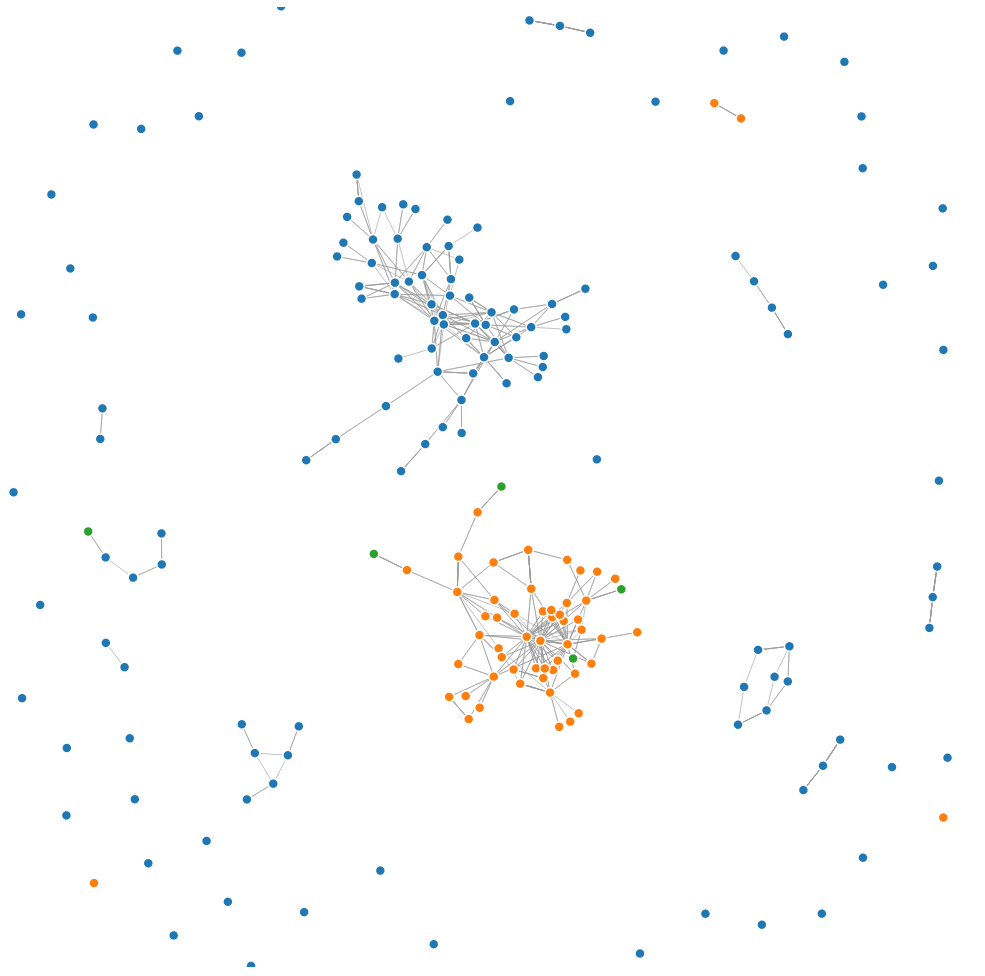
\includegraphics[width=\linewidth]{../Visualisation/screenshots/draft-fd-graph.png}
    \caption{Initial Force-Directed draft}
\end{figure}

Interestingly, the CS-modules form a more circle-layered structure, compared to
the Biology-modules which form two `clusters' and several small `constellations'
of modules. This is because CS has more core modules which then enable a lot of
different topic, whereas Biology splits into two `factions' (molecular and
medicinal) early on. There are also some modules which are completely disjoint
from the network. These are mostly 5000-level PGT master modules, along with
some gateway modules.
\begin{figure}
    \centering
    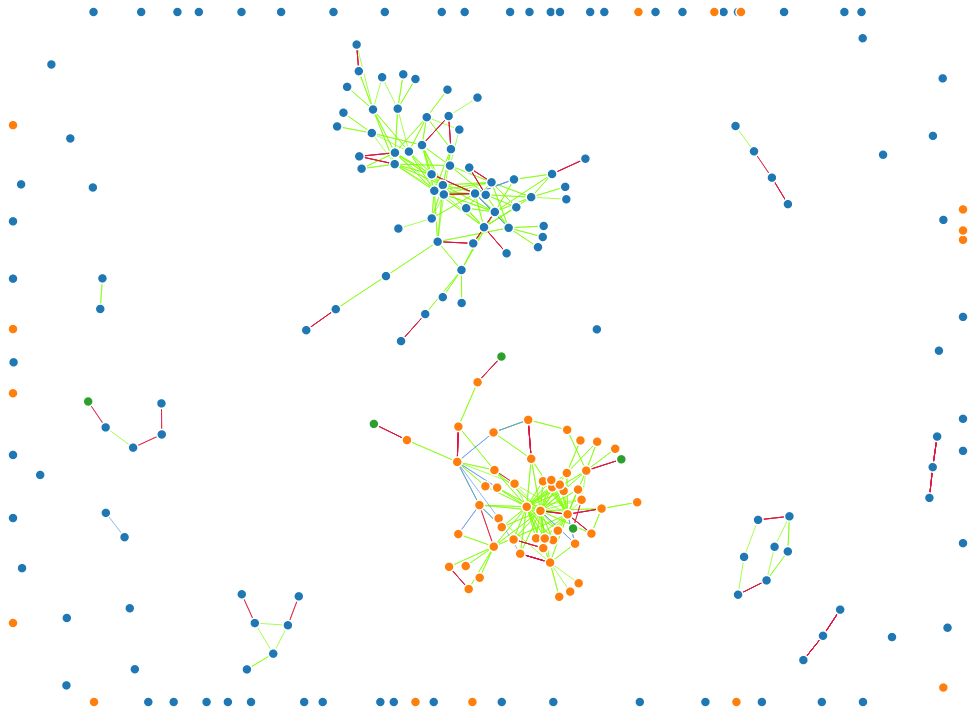
\includegraphics[width=0.8\linewidth]{../Visualisation/screenshots/draft-fd-colour.png}
    \caption{Force-Directed draft with colour-coded links and bounded area}
\end{figure}

I then modified this example to take the type of requisites into account,
colour-coding them. I used green for pre-requisites, blue for co-requisites, and
red for anti-requisites. 
\begin{figure}
    \centering
    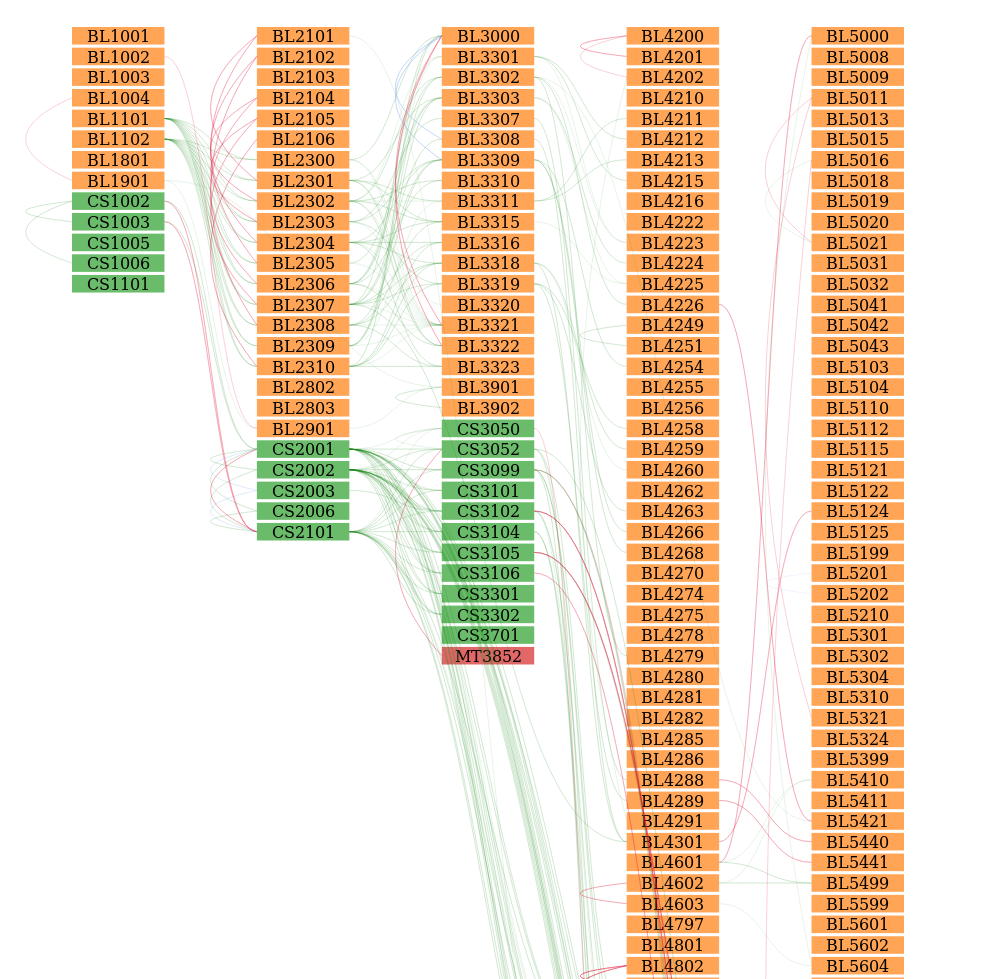
\includegraphics[width=\linewidth]{../Visualisation/screenshots/draft-columns.png}
    \caption{Initial column-oriented draft}
\end{figure}

Having familiarised myself with D3 and data-handling, I created a
column-oriented draft. Once it was ready, I took it and used it to create the
final visualisation.

\section{Column-oriented Layout}
    \subsection{Idea}
    The idea of the column-oriented layout was that each column would represent
    a level, 1000-5000. I considered having columns per semester. However, this
    would require some nodes to have double-width for whole-year modules and
    would further complicate how links between levels would be shown. Therefore,
    I decided against it and stuck with a column per level. The requisites would
    be smooth, colour-coded lines between the modules. The idea was that on
    hover/mouse-over, the links would show what modules the module selected
    en- or disabled, and if the person chose to take the module, what they would
    need to take before that.
    
    \subsection{Data pre-processing}
    To take full advantage of D3 and the DOM, I used D3-nest to nest both the
    modules and the requisites. The modules were nested by level, using a
    function which returned the 3rd character of their code, i.e. the level. The
    requisites were nested by their type.
    
    To be able to highlight the ancestors of a node, I needed a function which
    found these going back an arbitrary number of links with potential loops.
    This was a more problematic part of the project, and I eventually ended up
    with two solutions. The first was using a graph-library on the server-side
    and using it to find the ancestors of a node. The second was an idea by
    Iain Carson, which enabled me to do it client-side. By constructing a
    \texttt{Node} object in JavaScript and using it to represent each module, I
    could add a method to the prototype of the object, thereby causing all
    instances to have that method. The method itself, called
    \texttt{returnNodes}, checks whether the node that called it is already in
    the list of relevant nodes and if it is, returns. If the node is not in the
    list, it adds it, finds all the links and ancestors of that node, adds the
    links to the list of links traversed, and recursively calls itself on all
    the ancestor nodes. This results in the list of nodes eventually containing
    all the ancestors, and the list of links containing all links traversed to
    construct the node-list. These lists are then used to associate CSS-classes
    denoting ancestry with the relevant DOM-elements, which in turn allows the
    browser to immediately select all ancestors by finding which DOM-elements
    have the \texttt{ancestor-of-<Node>} class.
    
    \subsection{Visualisation using D3}
    The nodes are spaced out using D3's \texttt{scale\_band} method. This
    automatically also figures out the size of the bands, and allows specifying
    what percentage of the band should be padding. For the width, I set this to
    50\%, i.e. the space between each column should be 1 column-width, and I set
    the space between each row to be 15\%, based on experimentation.
    \\
    
    Each level in the nodes and edges have an SVG-group associated with them.
    This allows for easy translation of the columns and also allows the
    developer to easily inspect the relevant elements in the browser. A
    rectangle is drawn for each node, using the band-scales to determine width
    and height. Each \texttt{rect}'s fill colour is determined by the school,
    using the default D3 10-hue categorical colour scale,
    `\texttt{d3.schemeCategory10}'. The module code is then put as
    \texttt{text} in the center of the \texttt{rect}, towards the bottom. This
    is not a perfect solution, however, centering the text in the box is
    difficult due to the \texttt{rect}'s coordinates referring to the top-left
    corner of the rect, whereas the \texttt{text}'s coordinates, when centering,
    refer to the bottom-center of the text (and bottom-left when not
    centering). Taking the font-height into account is near-impossible, due to
    what browsers use which default font and whether users have changed that,
    and therefore, placing the \texttt{text} at the center of the \texttt{rect},
    towards the bottom seemed like the best approach.
    \\
    
    The links are drawn using cubic bezier curves. To make the endpoints match
    with the edges of a \texttt{rect} instead of always using the top-left
    corner, the width and height is taken into account. The path can be
    calculated using the D3 horizontal cubic bezier curve generator,
    `\texttt{d3.linkHorizontal()}', with the `horizontal' bit referring to the
    direction of the tangents of the cubic bezier links. This generator returns
    a series of SVG-path commands used to draw the line. If the link is between
    two modules in the same column, the path is instead calculated manually to
    achieve an arc (using a quadratic bezier line) rather than a straight line,
    which is what the generator returns in this case.
    
    \subsection{Styling and Interactivity}
    SVG-paths default to constructing a closed loop with a fill between the
    lines. Therefore, the fill is set to \texttt{none}. To make the
    highligthting ``pop'' more, the nodes and links have a lower opacity by
    default. Due to the large number of links and their overlapping, links have
    a minimally visible opacity of $0.1$. Any \texttt{highlighted}-classed nodes
    and links have increased opacity and the nodes also have a black outline.
    
    When a node is moused over, the \texttt{highlighted} class is added to all
    ancestor nodes and all links involved in this, resulting in them being
    highlighted. When the mouse then leaves the node, all
    \texttt{highlighted} classes are removed from the DOM-elements containing
    them.
